\documentclass[a4paper]{article}
\usepackage{parskip}
\usepackage[utf8]{inputenc}
\usepackage[norsk]{babel}
\usepackage{tikz,pgfplots}
\usepackage{amsmath}
\usepackage{soul}
\usepackage[font={small,it},labelfont=bf]{caption}
%\usepackage[none]{hyphenat}
\usepackage{booktabs}

%TiKz
\usepackage{tikz,pgfplots}


%Pgf
\usepackage{pgf}
\usepackage{pgffor}

\newlength\figureheight 
\newlength\figurewidth 
\newcommand{\tikzfig}[3]{\footnotesize 
\setlength\figurewidth{#2} 
\setlength\figureheight{#3}
\input{#1.tikz}}
\pgfplotsset{compat=newest}

%Pdf_tex
%\usepackage{transparent}
%\newcommand{\pdftex}[2]{\footnotesize
%\def\svgwidth{#2}
%\input{#1.pdf_tex}}

%\usepackage[left=4cm,right=4cm,top=4cm,bottom=4cm]{geometry}
\title{Eksperimentell bestemmelse av nødvendig nedkjølingstid for vørter}
\date{25.10.14}

%TASK
\newcommand{\task}[3]{\vskip 2em \tikz[baseline=(char.base)]{\node[shape=circle,draw,inner sep=2pt](char) {\textbf{#1}};} \textbf{#2} \vskip 0.2em \textit{#3} \vskip 0.2em}

\begin{document}
\maketitle

\section{Introduksjon}
Når man lager øl trengs vørter. Vørteren må kokes, men gjæren kan ikke tilsettes før vørteren er kald igjen. Nedkjølingen av kokt vørter bør gå så fort som mulig; en vørterkjøler er fryktelig fin å ha når øl skal brygges. For å estimere nødvendig kjølningstid av vørter som holder 100 grader, ble det gjennomført et forsøk av nedkjøling av vann med en kjøler levert av {\textsc{Kvålstabø Kjølermakeri}$^{\text{TM}}$}.

\section{Laboppsett og beskrivelse av eksperiment}
En kjele ble fylt med 25 liter vann, tilsvarende dimensjonert vørtermengde for kjøleren. Vannet i kjelen hadde en initiell temperatur på 47 grader. Romtemperaturen under forsøket var behagelige 23 grader, mens innførselstemperaturen på vannet holdt gufne 9 grader. Eksperimentet ble avsluttet etter 32 minutter, da vannet i kjelen holdt 11 grader. Laboppsettet er vist i figur \ref{fig:Foto1} og \ref{fig:Foto2}.

\begin{figure}
\centering
\includegraphics[width=\linewidth]{2.jpg}
\caption{Hyttekjele fylt med vann og vørterkjøler i aksjon. Rotete kjøkken er påkrevd.}
\label{fig:Foto1}
\end{figure}

\begin{figure}
\centering
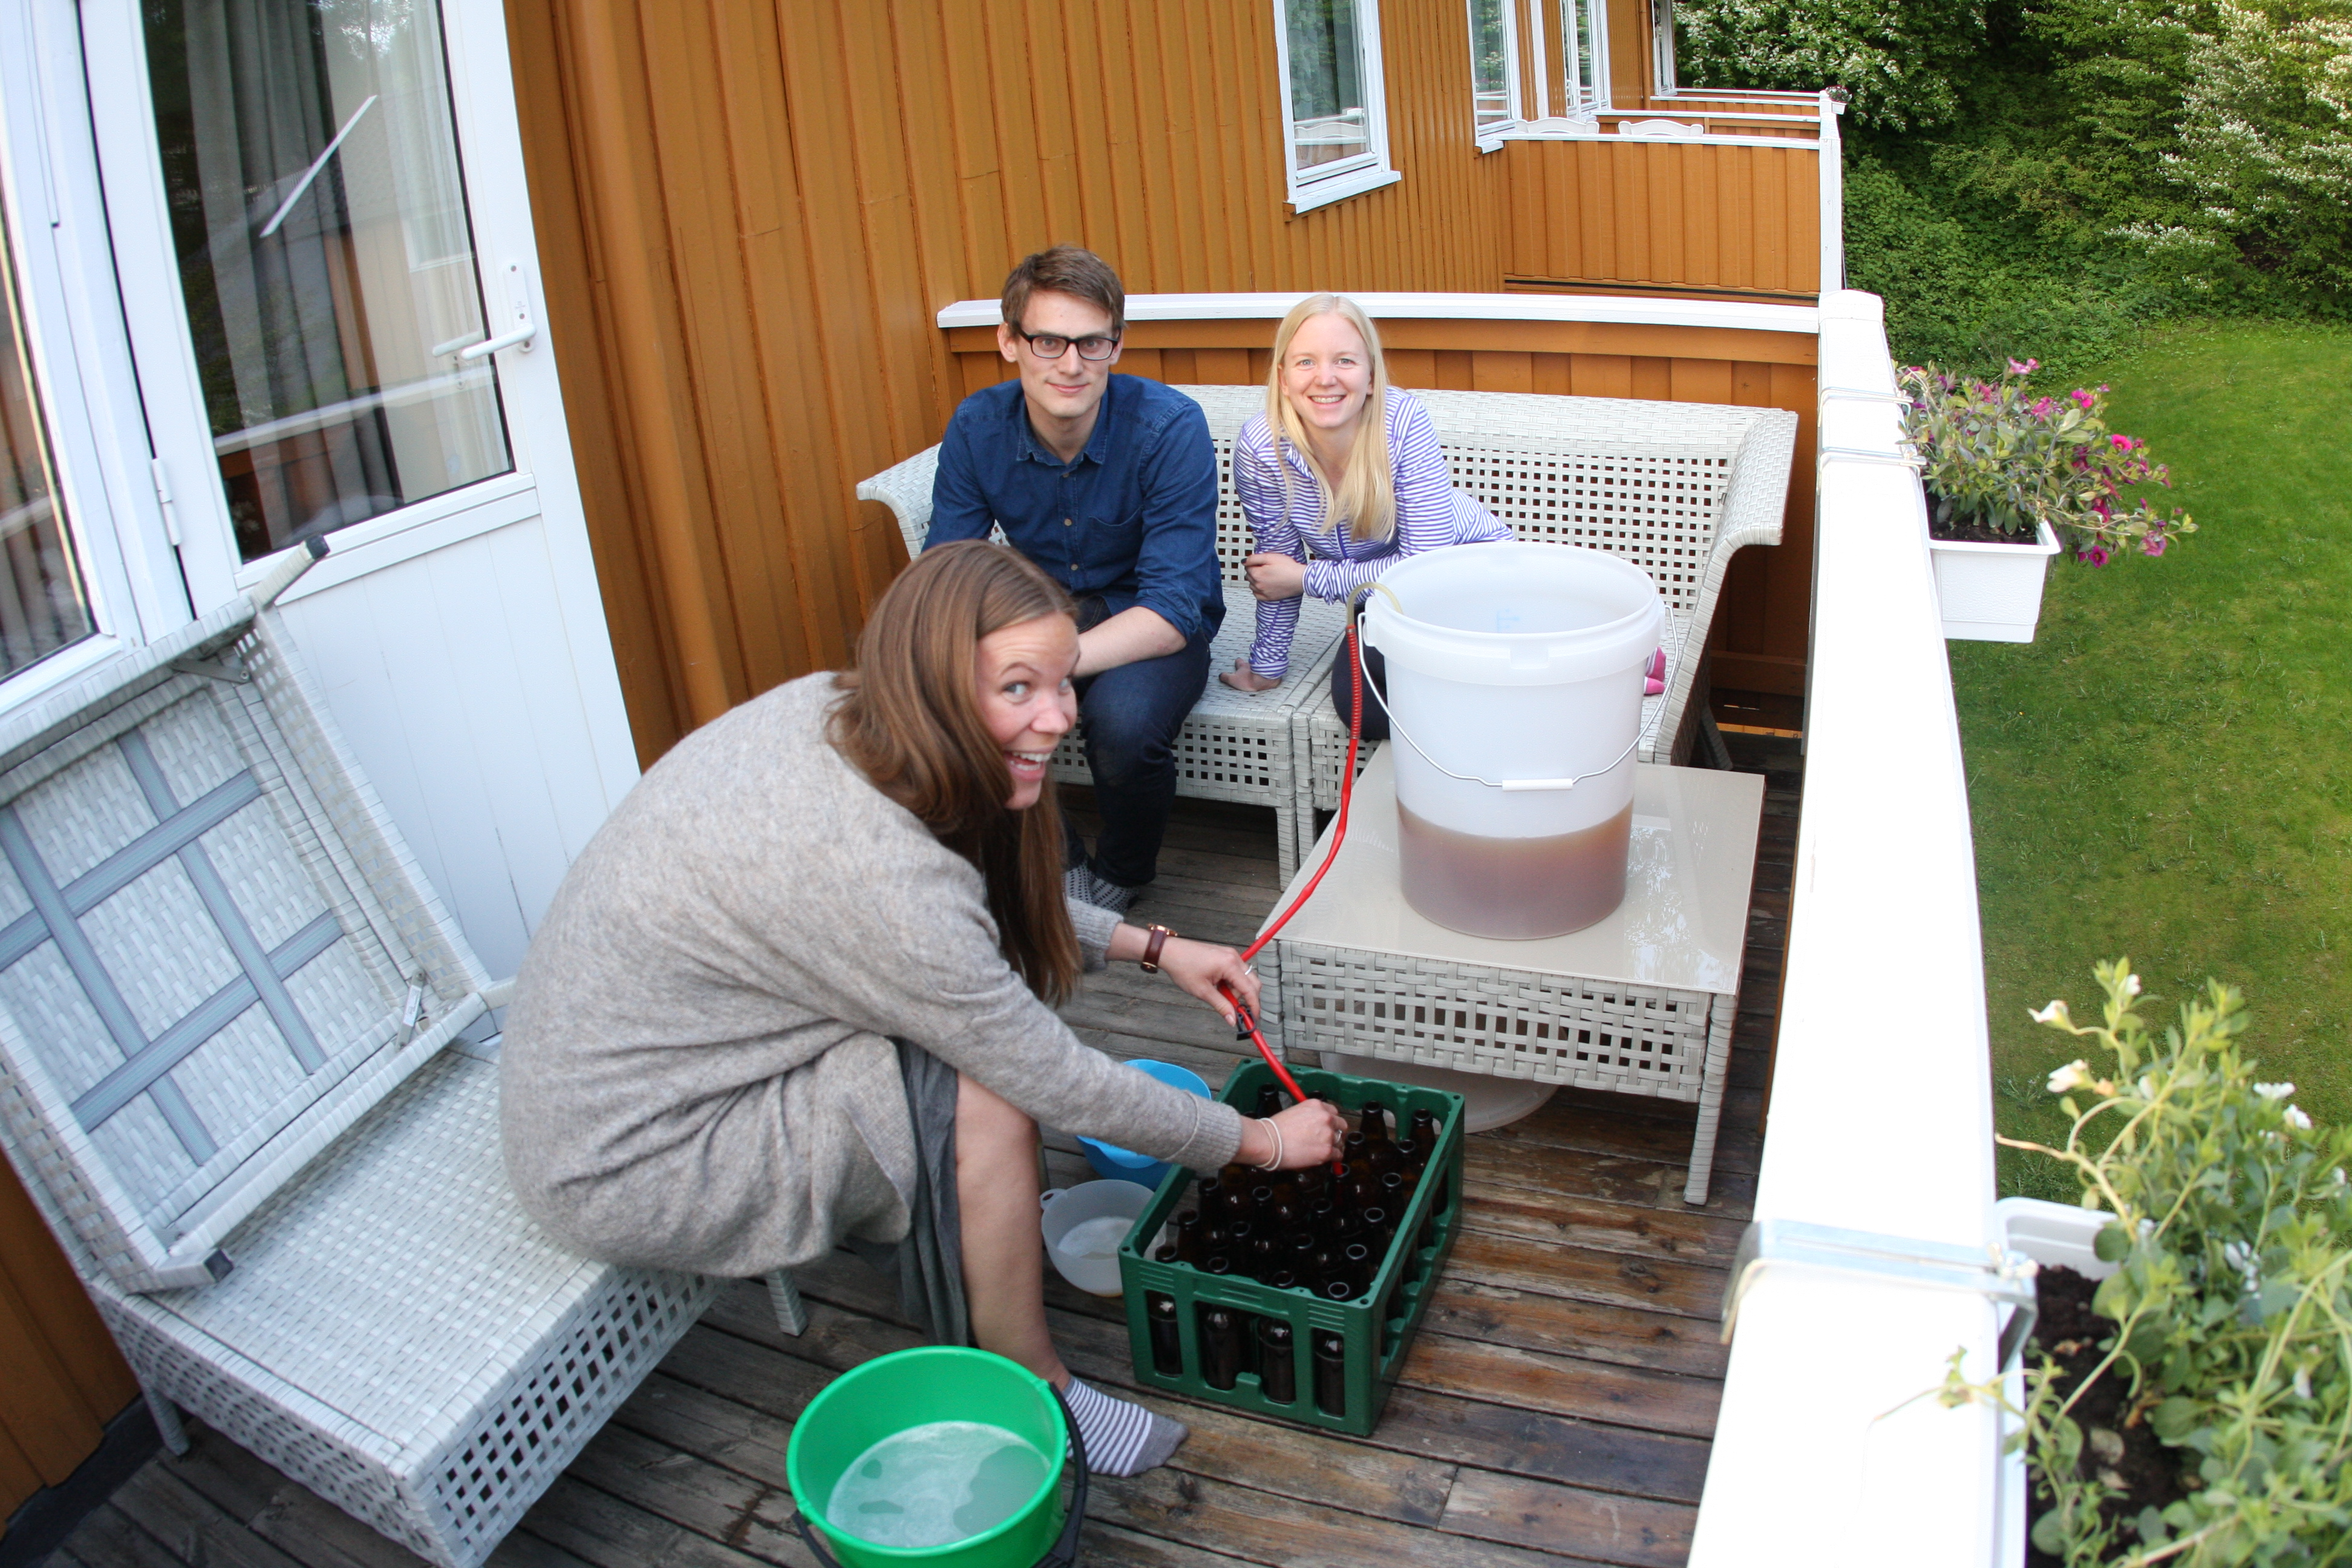
\includegraphics[angle=-90, width=0.7\linewidth,trim=0 0 10cm 0,clip]{1.jpg}
\caption{Digitalt avlesningsapparat for temperaturmåling plassert i kjelen under forsøket.}
\label{fig:Foto2}
\end{figure}

\section{Teori, resultat, diskusjon og konklusjon}
De tre første målepunktene ble sett bort i fra, og en minste-kvadraters kurvetilpasning gjennomført på de resterende punktene. Kurvetilpasningen var basert på følgende matematiske modell:
\begin{equation}
T = a+b\cdot \exp(c\cdot t)
\end{equation}
hvor $T$ er temperatur i Celsius, $t$ er tid, og $a$, $b$ og $c$ er parameterne som skal tilpasses. Kurvetilpasningen ga følgende funksjon for temperaturforløpet:
\begin{equation} \label{eq:T}
T = 9.09 + 34.9 \exp(-0.0882 \bar{t})
\end{equation}
Målepunktene og kurvetilpasningen er vist i figur \ref{fig:Fig1}. Parameterne bestemt over baserer seg på at $\bar{t}=0$ når temperaturen holder 47 grader (starttemperatur). I en reell ølbryggingssituasjon vil vørteren holde 100 grader, og et uttrykk for temperaturen gitt $t=0$ ved 100 grader er derfor mer nyttig. For å oppnå dette innføres følgende sammenheng:
%
\begin{equation} \label{eq:tshift}
t=\bar{t} - t_{43^\circ\text{C}}
\end{equation}
hvor $t_{43^\circ\text{C}}=10.84 \text{min}$ er bestemt ved å løse ut for $t$ når likning \ref{eq:T} er satt lik 100. Ved å kombinere likning \ref{eq:T} og \ref{eq:tshift}, kunne følgende funksjon for temperaturforløpet bestemmes:
\begin{gather}
T = 9.09 [1 + 10 \exp(-0.0882 t)]
\end{gather}

\begin{figure}
\centering
\tikzfig{Fig1}{0.75\linewidth}{5cm}
\caption{Kurvetilpasning av måledata.}
\label{fig:Fig1}
\end{figure}

\begin{figure}
\centering
\tikzfig{Fig2}{0.75\linewidth}{5cm}
\caption{Forskjøvet kurvetilpasning.}
\label{fig:Fig2}
\end{figure}
%
Denne funksjonen er illustrert i figur \ref{fig:Fig2} sammen med innførselstemperatur på vannet og måltemperatur for vørteren. Ved å løse likningen over gitt $T=T_{\text{vørter}} = 20 ^\circ\text{C}$ for $t$, kunne nedkjølingstiden for 25 liter vørter ved 100$^\circ$C estimeres til \textit{24 minutter}.
\end{document}
